\section{Morte Stellare}\label{sec:morte-stellare}
\subsection{Nane Bianche}\label{sec:nane-bianche}
Per stelle con massa $M < 8\si{\solarmass}$, in seguito al collasso gravitazionale del nucleo, dovuto all'assenza di reazioni termonucleari, la densità aumenta vertiginosamente raggiungendo $\rho \sim \SI{e6}{g.cm^{-3}}$. In queste condizioni si raggiunge l'equilibrio idrostatico tra pressione gravitazionale e pressione degli elettroni degeneri.

Nel caso di nuclei a Carbonio e Ossigeno, è presente un sottilissimo strato non degenere di Elio ($M_{He} \sim 10^{-2} M_{WD}$)ed uno ancora più sottile di Idrogeno ($M_{H} \sim 10^{-4} M_{WD}$), sempre non degenere. Il prototipo di stella Nana Bianca è Sirius B, lontana da noi quasi $8.6 \si{ly}$ e con le caratteristiche mostrate in tabella~\ref{tab:sirius-b}.

\begin{table}
    \centering
    \caption{Nella tabella sono indicate le proprietà del corpo celeste noto come Sirius B, una nana bianca delle dimensioni simili a quelle terrestri, ma con massa comparabile con quella del sole, rendendolo un corpo estremamente denso.}\label{tab:sirius-b}
    \begin{tabular}{c|c}
        \toprule
        Proprietà & Valori\\
        \midrule
        M & $\sim 1.05 \si{\solarmass}$\\
        R & $\sim \SI{5.5 e8}{cm}$\\
        $\rho$ & $\sim \SI{e6}{g.cm^{-3}}$\\
        T & $\sim \SI{2.7}{K}$\\
        \bottomrule
    \end{tabular}
\end{table}

Nel bilanciamento tra la forza gravitazionale e la pressione elettronica degenere la relazione che emerge
\[
    M^{frac{1}{3}}R = 3\times 10^{19}
\]
mostrando che maggiore è la massa iniziale di una stella minore sarà la sua dimensione quando raggiungerà la forma di nana bianca. Questa relazione è stata ottenuto tenendo conto do effetti dovuti alla relatività generale, la quale ci permette inoltre di trovare un limite al valore che la massa di elettroni degeneri può sopportare, chiamata massa di Chandrasekhar e con valore $M_{Ch} = 1.44\si{\solarmass}$. In realtà la relazione che permette di trovare tale limite dipende dall'abbondanza di Idrogeno nella nana bianca, cioè:
\[
    M_{Ch} = 1.44(1+X)^2 \si{\solarmass}
\]
Ma questa relazione non vale solo per questo tipo di corpi, ma per tutte le strutture cosmiche esistenti tenute in equilibrio dalla pressione di elettroni degeneri, come ad esempio per Nane Bianche di Elio (He Nane Bianche).

Supponendo che la massa di una nana bianca rimanga costante nel corso della sua evoluzione, così come il raggio, si osserva che la luminosità diminuisce assieme alla temperatura, in figura~\ref{fig:WD} è mostrato l'andamento di questi corpi nel piano H-R a seconda della massa iniziale. L'evoluzione di una nana bianca risulta quindi parallela alle curve a raggio costante nel diagramma durante la sequenza di raffreddamento.
\begin{figure}
    \centering
    \subfloat[]{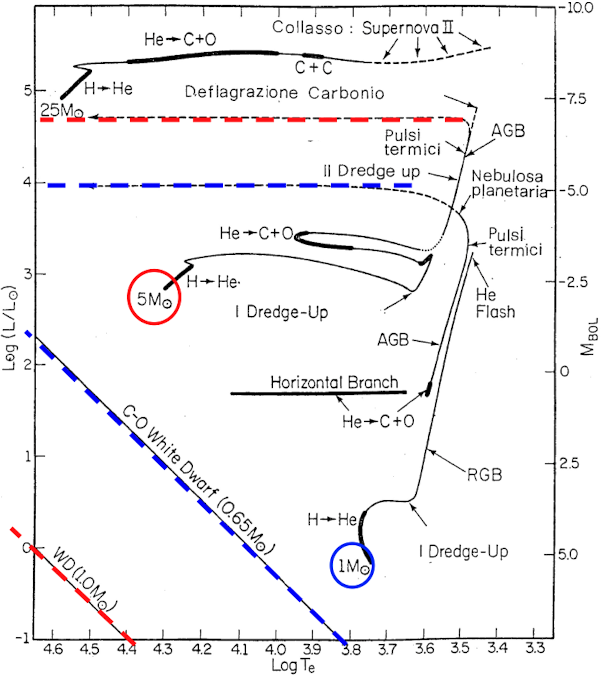
\includegraphics[width = 0.45\textwidth]{immagini/WD1.png}} \qquad
    \subfloat[]{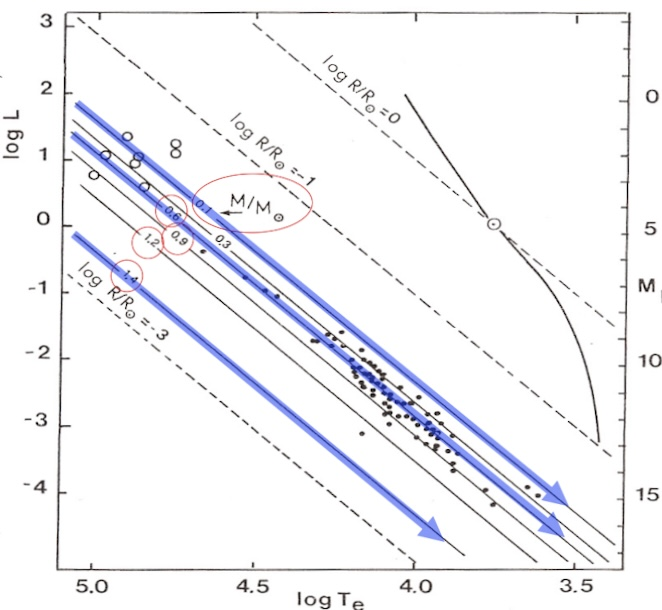
\includegraphics[width = 0.45\textwidth]{immagini/WD2.png}}
    \caption{}\label{fig:WD}
\end{figure}

La luminosità di questi copri sicuramente non sarà dovuta alla presenza di reazioni termonucleari o all'energia gravitazionale dovuta alla compressione, ma all'energia interna, principalmente termica, degli ioni. In particolare l'energia interna di una nana bianca è data dalla relazione:
\[
    U = \frac{M_{WD}}{A \cdot M_{H}} \frac{3}{2} k T_c
\]
e rappresenta una sorta di serbatoio di energia per essa, che viene adoperata durante la sua esistenza. In questo tipo di corpi il trasferimento di energia da una sezione all'altra va per conduzione.

I tempi di raffreddamento per una stella nana bianca seguono un andamento dato dalla relazione
\begin{equation}
    t_{cool} = 8.8\times 10^6 \left(\frac{M}{\si{\solarmass}} \right)^{\frac{5}{7}} \left( \frac{L}{\si{\solarluminosity}} \right)^{-\frac{5}{7}} \mbox{ yr}
\end{equation}
osservando che a luminosità fissate, minore sarà il tempo necessario a raffreddarsi. Ad esempio una nana bianca con luminosità costante a $L = 10^{-4.5} \si{\solarluminosity}$ a seconda che la massa sia $M = 1\si{\solarmass}$ o $M = 0.5 \si{\solarmass}$, il tempo di raffreddamento varia da $\SI{12e9}{yr}$ a $\SI{7.6e9}{yr}$.

\subsection{}